\documentclass[12pt, a4paper]{article}

\voffset=-1.5cm
\oddsidemargin=0.0cm
\textwidth = 470pt

\usepackage{epsfig}
\usepackage{subfigure}
%\usepackage{amscd}
\usepackage{amssymb}
\usepackage{amsbsy}
\usepackage{amsthm}
%\usepackage[dvips]{graphicx}
\usepackage{natbib}
\usepackage{framed}
\bibliographystyle{chicago}



\begin{document}
	\author{Kevin O'Brien}
	\title{MA4605}
	
	\tableofcontents \setcounter{tocdepth}{2}
	%-------------------------------------------------
\newpage
\Large	
\section{Chemometrics : Introduction to Module}
\begin{itemize}
\item Kevin O'Brien
\item email: kevin.obrien@ul.ie
\end{itemize}
\newpage
\subsection{Quantitative nature of analytical chemistry}
\begin{itemize}
\item Modern analytical chemistry is overwhelmingly a quantitative science.
A quantitative answer is much more valuable than a qualitative one.
\item It may be useful for an analyst to claim to have detected some boron in a
distilled water sample, but it is much more useful to be able to say how
much boron is present.

\item Often it is only a quantitative result that has any value at all.For
example, almost all samples of (human) blood serum contain albumin;
the only question is, how much ? Even where a qualitative answer is required, quantitative methods are
used to obtain it.

\item Quantitative approaches might be used to compare two soil samples. For example, they might be subjected to a particle
size analysis, in which the proportions of the soil particles falling within a number say 10, of particle-size ranges are determined. 
\item Each sample would then be characterized by these 10 pieces of data, which could
then be used to provide a quantitative assessment of their similarity.
\end{itemize}
\newpage

\begin{framed}
\begin{quote}

The extremely rapid development of analytical techniques in biology and
chemistry has left data analysis far behind, and as a result the statistical
analysis and interpretation of the data has become a major bottleneck in the
pipeline from measurement to information. \\ \noindent (Quote from ``Chemometrics with \texttt{R}", R. Wehrens,  Springer Use\texttt{R}! Series).
\end{quote}
\end{framed}

\newpage
\subsection{Learning Outcomes}
\begin{itemize}
	\item To give students a clear understanding of the importance of statistical methods in their work.
	\item To introduce students to the most widely used statistical techniques in the chemical process industries.
	\item To develop skills in the use of these techniques through actual case studies using statistical software packages
\end{itemize}
%=====================================================%


\subsection{Statement of Syllabus}
\begin{enumerate}
	\item \textbf{Hypothesis testing} - type I  and type II error, one and two-tailed tests, oc curves.
	\item \textbf{Statistical process control} - various charts, mean/range, individuals/moving range, cusum charts.
	\item \textbf{Capability studies} - capability indices.
	\item \textbf{Correlation and Regression} - method of least squares, multiple regression, linear and non-linear models, regression analysis, analysis of residuals.
	\item \textbf{Data Visualization} - Importance of plotting data.
	\item \textbf{Design of experiments and analysis of variance} - one and two way ANOVA, interaction, factorial designs, responses and factors, Plackett-Burman design, response surface methodology.
\end{enumerate}
\newpage

\subsection{Revision of Science Maths 3}
\begin{itemize}
\item This module follows on from \textbf{Science Maths 3  - Introduction to Statistics MA4603} with Dr Joseph Lynch. 
\item If you could make some quick revisions of the course material there over the next three or four weeks that would be great.
\item We will not be doing much in the way of pen-and-paper calculations ( there will be a few questions here and there). 

\item For the first few classes, we will go back over the Normal Distribtion, Hypothesis Testing Correlation, Simple Linear Regression, P-values etc

\end{itemize}



\subsection{Text Books}

\noindent My own notes would be suffficient. I will publish them on SULIS. You can have a look at the folowing publications too.
\begin{itemize}
	\item[1.] Statistical Analysis Methods for Chemists (Author : William P Gardiner)
	\item[2.] simpleR - Using \texttt{R} for Introductory Statistics (Author : John Verzani)
	\item[3.] An Introduction to \texttt{R} (Authors: The R Project)
\end{itemize}

%-------------------------------------------------
\newpage
\section{Introduction to \texttt{R}}

\subsection{The \texttt{R} Project for Statistical Computing}
\begin{figure}[h!]
\centering
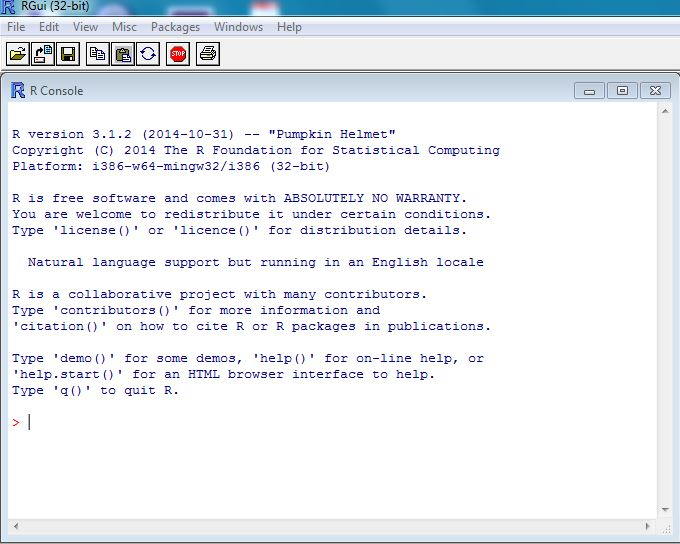
\includegraphics[width=0.60\linewidth]{Rscreenshot}
%\caption{}
%\label{fig:Rscreenshot}
\end{figure}

\noindent \texttt{R} is a language and environment for statistical computing and graphics. \texttt{R} provides a wide variety of statistical and graphical techniques, and is highly extensible. Among its tools
one can find implemented
\begin{itemize}
	\item linear and nonlinear modelling,
	\item classical statistical tests,
	\item time-series analysis,
	\item classification,
	\item clustering,
	\item ...and many more.
\end{itemize}

\newpage
\noindent One of R's strengths is the ease with which well-designed publication quality plots can be produced.
including mathematical symbols and formulae where needed.
\begin{itemize} \item
	\texttt{R} is a computing software for statistical analysis \item The package is available for all popular operating systems: Windows, Mac or Linux.
	\item It is free!
	\item Everyone (knowledgeable enough) can contribute to the software by
	writing a package.
	\item Packages are available for download through a convenient facility
	\item It is fairly well documented and the documentation is available either
	from the program help menu or from the web-site.
	\item It is the top choice of statistical software among academic statisticians
	but also very popular in industry specially among biostatisticians and
	medical researchers (mostly due to the huge package called
	Bioconductor that is built on the top of \texttt{R}).
	\item It is a powerful tool not only for doing statistics but also all kind of
	scientific programming.
\end{itemize}
\newpage

\noindent \texttt{R} is an integrated suite of software facilities for data manipulation, calculation and graphical display. It
includes
\begin{itemize}
	\item an effective data handling and storage facility,
	\item a suite of operators for calculations on arrays, in particular matrices,
	\item a large, coherent. integrated collection of intermediate tools for data analysis,
	graphical facilities for data analysis and display either on-screen or on hard-copy, and
	\item a well-developed, simple and effective programming language which includes conditionals, loops,
	user-defined recursive functions and input and output facilities.
\end{itemize}

\subsection{Downloading and Installing \texttt{R}}

\begin{itemize}
	\item \texttt{R} can be downloaded from the CRAN website: \textit{http://cran.r-project.org/}
	\item You may choose versions for windows, mac and linux.
	\item As per the instructions on the respective pages, you require the ``base" distribution.
	\item Now you can download the installer for latest version of \texttt{R} , version 3.2.1.
	\item Select the default settings. Once you finish, the \texttt{R} icon should appear on your desktop.
	\item Clicking on this icon will start up the program.
\end{itemize}

\subsection{Output Graphics from chemCal R package}
\begin{figure}[h!]
\centering
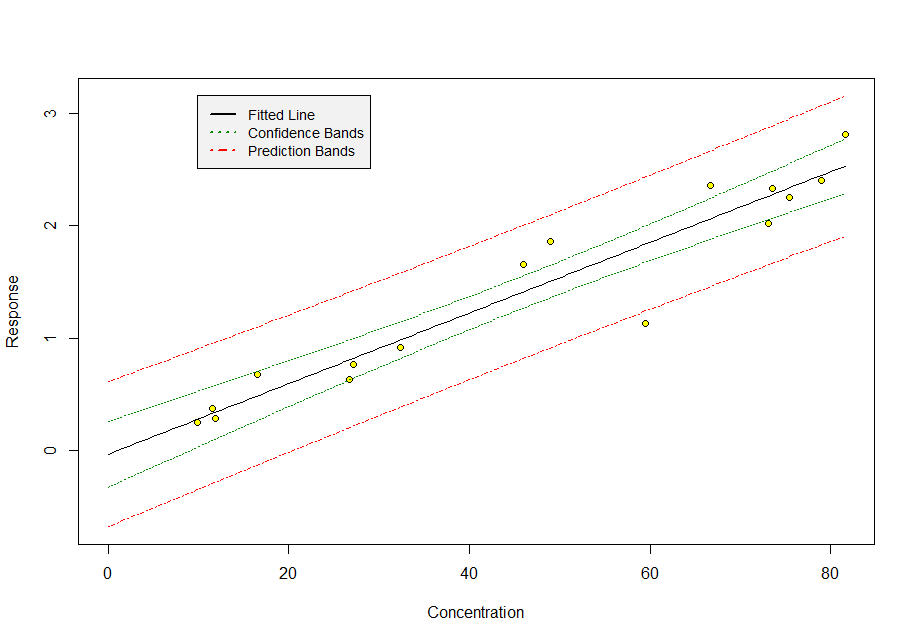
\includegraphics[width=0.9\linewidth]{ChemCal}
%\caption{}
%\label{fig:ChemCal}
\end{figure}

\noindent \textbf{Remark} Material covered in Simple Linear Regression will feature a lot.
\newpage

\subsection{Example of R Analysis: Titration experiment}
	
	Cosider the following titration experiment where 4 Students performing the same experiment five times, hence each yield 5 results. \vspace{0.5cm}
	%(Table 1.1 random and systematic errors).
	{
		\large
	\begin{tabular}{|c|ccccc|l|}
		\hline
		% after \\: \hline or \cline{col1-col2} \cline{col3-col4} ...
		Student & Results  & (ml) &  &  &  & Comment \\ \hline
		A & 10.08 & 10.11 &10.09 &10.10&10.12 & Precise, biased\\ \hline
		B & 9.88 &10.14& 10.02 &9.80& 10.21& Imprecise unbiased\\ \hline
		C & 10.19 &9.79& 9.69 &10.05& 9.78 & Imprecise, biased\\ \hline
		D & 10.04 &9.98 &10.02 &9.97 &10.04 & Precise, unbiased \\
		\hline
	\end{tabular}\\
	
}

\begin{figure}[h!]
\centering
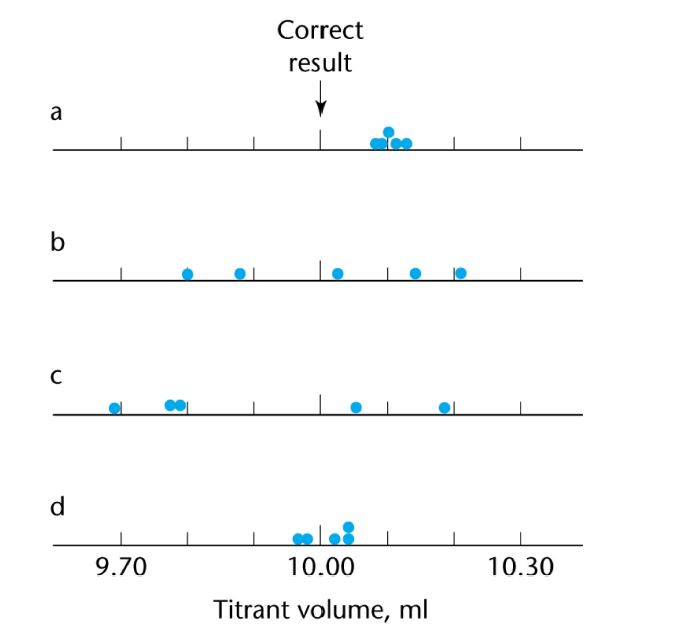
\includegraphics[width=0.8\linewidth]{Titra2}
%\caption{}
%\label{fig:Titra2}
\end{figure}
\newpage
\subsection{Measures of Centrality and Dispersion}	
Two criteria were used to compare these results, the average value (technically know
as a measure of centrality and the degree of spread (or dispersion). 	
\begin{itemize}
\item The average value
	used was the arithmetic mean (usually abbreviated to \emph{the mean}), which is the sum
	of all the measurements divided by the number of measurements.

\item	The mean, $\bar{x}$ , of $n$ measurements is given by \[ \bar{x}  = {\sum{x} \over n} \]
	
\item The dispersion (or spread) was measured by the difference between the highest and
	lowest values (i.e. the range). 
\item A more useful measure, which utilizes all the values, is the sample
	standard deviation, $s$, which is defined as follows:

	\[s=  \sqrt{ {\sum(x-\bar{x})^2 \over n-1} }   \]

\item Recall: variance is the standard deviation squared.
\item The coefficient of variation is the relative standard deviation (in
percentage)
\end{itemize}
\newpage
\subsection{Output of \texttt{R} Procedure}	
\begin{framed}
\begin{verbatim}
#Comuting means

apply(Titra,1,mean)

#       A      B      C       D
# 10.0950 9.9600 9.9300 10.0025

#and standard deviation

apply(Titra,1,sd)

#         A          B          C          D
#0.01290994 0.15055453 0.23036203 0.03304038
\end{verbatim}
\end{framed}
%======================================================%
\newpage
\section{Revision of Topics from MA4603}


\subsection{Statistical significance}

\begin{itemize}
\item \textbf{Statistical significance} is a mathematical tool used to determine whether the outcome of an experiment is the result of a relationship between specific factors or due to chance. Statistical significance is commonly used in the medical field to test drugs and vaccines and to determine causal factors of disease. Statistical significance is also used in the fields of psychology, environmental biology, and any other discipline that conducts research through experimentation.



\item Statistics are the mathematical calculations of numeric sets or populations that are manipulated to produce a probability of the occurrence of an event. Statistics use a numeric sample and apply that number to an entire population. 

%\item For the sake of example, we might say that $80\%$ of all irish adults drive a car. It would be difficult to question everybody about whether or not they drive a car, so a random number of people would be questioned and then the data would be statistically analyzed and generalized to account for everyone.



\item In a scientific study, a hypothesis is proposed, then data is collected and analyzed. The statistical analysis of the data will produce a number that is statistically significant if it falls below $5\%$, which is called the confidence level. In other words, if the likelihood of an event is statistically significant, the researcher can be $95\%$ confident that the result did not happen by chance.



\item Sometimes, when the statistical significance of an experiment is very important, such as the safety of a drug meant for humans, the statistical significance must fall below $3\%$. In this case, a researcher could be $97\%$ sure that a particular drug is safe for human use. This number can be lowered or raised to accommodate the importance and desired certainty of the result being correct.



\item Statistical significance is used to reject or accept what is called the null hypothesis. A hypothesis is an explanation that a researcher is trying to prove. The null hypothesis holds that the factors a researcher is looking at have no effect on differences in the data. 
\item Statistical significance is usually written, for example, \[...t=.02, p<.05...\]Here, "t" stands for the statistic test score and "p<.05" means that the probability of an event occurring by chance is less than $5\%$. These numbers would cause the null hypothesis to be rejected, therefore affirming that the alternative hypothesis is true.
%
%
%
%\item Here is an example of a psychological hypothesis using statistical significance: It is hypothesized that baby girls smile more than baby boys. In order to test this hypothesis, a researcher would observe a certain number of baby girls and boys and count how many times they smile. At the end of the observation, the numbers of smiles would be statistically analyzed.



%\item Every experiment comes with a certain degree of error. It is possible that on the day of observation all the boys were abnormally grumpy. The statistical significance found by the analysis of the data would rule out this possibility by 95\% if t=.03. In this case, the null hypothesis that baby girls do not smile more than baby boys would be rejected, and with 95\% certainty, the researcher could say that girls smile more than boys.
%\item 
\end{itemize}


\newpage
\subsection{Hypothesis testing: introduction}

\begin{framed}
	\begin{quote}
		
		“The process by which we use data to answer questions about parameters 	
		is very similar to how juries evaluate evidence about a defendant.” –\textit{from
			Geoffrey Vining, Statistical Methods for Engineers, Duxbury, 1st edition, 1998.}
		
	\end{quote}
\end{framed}

The objective of hypothesis testing is to access the validity of a claim against a counterclaim using sample data

\begin{itemize}\item The claim to be “proved” is the alternative hypothesis($H_1$).\item The competing claim is called the null hypothesis($H_0$).\item One begins by assuming that $H_0$ is true. \end{itemize}

\vspace{0.5cm}

\noindent 
If the data fails to contradict $H_0$ beyond a reasonable doubt, then $H_0$ is not rejected (recall - we would say "fail to reject" rather ``accept"). 

However, failing to reject $H_0$ does not mean that we accept it as true. It simply means that $H_0$ cannot be ruled out as a possible explanation for the observed data.
%A proof by insufficient data is not a proof at all.


\newpage

%===============================================================================================%



\begin{itemize}

\item Hypothesis testing is a common practice in science that involves conducting tests and experiments to see if a proposed explanation for an observed phenomenon works in practice. 
\item A hypothesis is a tentative explanation for some kind of observed phenomenon, and is an important part of the scientific method. The scientific method is a set of steps that is commonly employed by those in scientific fields to give scientific explanations for various phenomena.



%\item Any tentative explanation can be referred to as a hypothesis if it can be submitted to hypothesis testing. There are, however, a set of guidelines for an explanation to be considered a true scientific hypothesis. The first major point is testability; a scientific hypothesis must be able to proceed to the stage of hypothesis testing to be considered a scientifically legitimate hypothesis. 

%\item It is generally suggested that a hypothesis be relatively simple, though this is not always possible. Hypotheses must also be able to explain the phenomena under any set of conditions; if a hypothesis can only explain a phenomenon in one set of conditions, it is generally considered unacceptable.


%
%\item Hypotheses are generally considered useful only if they are likely to improve on the current body of knowledge on a subject and pave the way for greater knowledge to be acquired in the future. Also, a hypothesis is generally not acknowledged if it defies other commonly recognized knowledge. If a hypothesis meets all of these requirements, it will typically proceed to the hypothesis testing phase.

%
%
%\item In hypothesis testing, the testers seek to discover evidence that either validates or disproves a given hypothesis. Usually, this involves a series of experiments being conducted in many different conditions. If the hypothesis does not stand up to the tests in all conditions, something is usually wrong with the hypothesis and a new one must be formed to take the new information into account. 
%\item The new hypothesis is submitted to the same hypothesis testing. If it passes and is not proven wrong, it can eventually be considered a scientific theory or law, though nothing in science can be proven to be absolutely true.



\item One common method of hypothesis testing is known as \textbf{statistical hypothesis testing}, and typically deals with large quantities of data. 
\item Experiments and tests are conducted and the data is collected. If the data collected shows that it is unlikely that the results occurred by chance, it is considered statistically significant and can be used to support a hypothesis.
\item The results of hypothesis tests are often expressed in terms of $p-$values.
\end{itemize}
\newpage

\subsection*{Interpreting $p-$values}

For the purposes of this module, we will use the following rules of thumb.
If we do not have a significant $p-$value, we fail to reject the null hypothesis.
If we have a significant result, we reject the Null Hypothesis.
\begin{itemize}
	\item p-value is greater than 0.05 - Not Significant
	\item p-value is between 0.05 and 0.01 - Significant
	\item p-value is between 0.01 and 0.001 - Very Significant
	\item p-value is less than 0.001 - Highly Significant
\end{itemize}
\newpage


\noindent \textbf{Example 1}
\begin{figure}[h!]
\centering
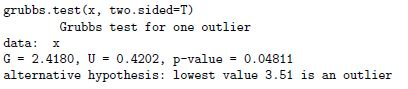
\includegraphics[width=0.9\linewidth]{gruubsTest}
\caption{}
\label{fig:gruubsTest}
\end{figure}

\bigskip
\noindent \textbf{Example 2}
\begin{figure}[h!]
\centering
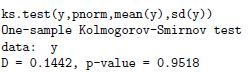
\includegraphics[width=0.6\linewidth]{kstest}
\caption{}
\label{fig:kstest}
\end{figure}


\end{document}


